\chapter{Results}
\label{ch:results}

Over the course of the internship many different parameters had to be determined and set up for the final demo. This chapters documents the results of all the experiments performed as well as the final demo of the working setup.

\section{Over-the-air User Data Transmission}\label{sec:OTADataTrans}

Following the data transmission through over the air using LTE AFW, benchmarks were run to check the loss of data over the wireless medium. Data loss tests were profiled using \textit{iperf}, a software used to profile UDP traffic.

A server and client of the version of the iperf application was used to test the wireless interface. Where the data was produced by the client on UDP port \texttt{50000} and received on the localhost \texttt{127.0.0.1} on UDP port \texttt{60000} once a SISO and MIMO Tx-Rx wireless interface was setup for the respective tests. The version of iperf used is shown below.

\begin{lstlisting}[style=DOS]
iperf version 2.0.9 (1 June 2016) pthreads
\end{lstlisting}

The command used to start up a Client is shown below.
\begin{lstlisting}[style=DOS]
iperf.exe -c 127.0.0.1 -u -i 1 -b 10M -t 10 -p 50000
\end{lstlisting}

The command used to start up a server is shown below.
\begin{lstlisting}[style=DOS]
iperf.exe -s -u -B 127.0.0.1 -i 1 -p 60000
\end{lstlisting}

\subsection{SISO}\label{ssec:SISOOTA}

A SISO communications channel was setup with the Tx and Rx settings as mentioned in Table \ref{tab:TXUSRPParam} and \ref{tab:RXUSRPParam} using the LTE AFW template. On conducting UDP data flow tests, it was observed that there were no packet drops with a UDP data block loss rate of $0\%$.

As a next step a short video clip was fed into the UDP stream of the transmitter and received with no video and audio frame drops at all. The demo video can be seen here \footnote{\url{https://drive.google.com/file/d/1PFWkfSUSSI4UC-m7nrF5EjYPyTy7iTYG/view?usp=sharing}}.

\subsection{MIMO}\label{ssec:MIMOOTA}

In the second test a MIMO communications channel was setup with the Tx and Rx settings as mentioned in Table \ref{tab:TXUSRPParam} and \ref{tab:RXUSRPParam} using the LTE MIMO AFW 2x2 extention software. On conducting UDP data flow tests, it was observed that there were large packet losses with a UDP data block loss rate of around $25\%$. Below is an output of the server client iperf application.


\begin{lstlisting}[style=DOS]
Microsoft Windows [Version 10.0.18363.1016]
(c) 2019 Microsoft Corporation. Alle Rechte vorbehalten.

C:\Users\ge69mog>cd Downloads\iperf-2.0.9-win64\iperf-2.0.9-win64

C:\Users\ge69mog\Downloads\iperf-2.0.9-win64\iperf-2.0.9-win64>iperf.exe -s -u
-B 127.0.0.1 -i 1 -p 60000
------------------------------------------------------------
Server listening on UDP port 60000
Binding to local address 127.0.0.1
Receiving 1470 byte datagrams
UDP buffer size:  208 KByte (default)
------------------------------------------------------------
[  3] local 127.0.0.1 port 60000 connected with 127.0.0.1 port 49721
[ ID] Interval       Transfer     Bandwidth        Jitter   Lost/Total Datagrams
[  3]  0.0- 1.0 sec   996 KBytes  8.16 Mbits/sec   2.017 ms  166/  860 ((*@\textcolor{red}{19\%}@*))
[  3] 0.00-1.00 sec  50 datagrams received out-of-order
[  3]  1.0- 2.0 sec   904 KBytes  7.41 Mbits/sec   2.426 ms  227/  857 ((*@\textcolor{red}{26\%}@*))
[  3] 1.00-2.00 sec  70 datagrams received out-of-order
[  3]  2.0- 3.0 sec   902 KBytes  7.39 Mbits/sec   2.148 ms  219/  847 ((*@\textcolor{red}{26\%}@*))
[  3] 2.00-3.00 sec  61 datagrams received out-of-order
[  3]  3.0- 4.0 sec   916 KBytes  7.50 Mbits/sec   1.904 ms  222/  860 ((*@\textcolor{red}{26\%}@*))
[  3] 3.00-4.00 sec  69 datagrams received out-of-order
[  3]  4.0- 5.0 sec   871 KBytes  7.14 Mbits/sec   4.137 ms  206/  813 ((*@\textcolor{red}{25\%}@*))
[  3] 4.00-5.00 sec  56 datagrams received out-of-order
[  3]  5.0- 6.0 sec   953 KBytes  7.81 Mbits/sec   4.710 ms  226/  890 ((*@\textcolor{red}{25\%}@*))
[  3] 5.00-6.00 sec  86 datagrams received out-of-order
[  3]  6.0- 7.0 sec   828 KBytes  6.79 Mbits/sec   2.786 ms  253/  830 ((*@\textcolor{red}{30\%}@*))
[  3] 6.00-7.00 sec  84 datagrams received out-of-order
[  3]  7.0- 8.0 sec   843 KBytes  6.90 Mbits/sec   4.467 ms  250/  837 ((*@\textcolor{red}{30\%}@*))
[  3] 7.00-8.00 sec  90 datagrams received out-of-order
[  3]  8.0- 9.0 sec   970 KBytes  7.95 Mbits/sec   1.648 ms  200/  876 ((*@\textcolor{red}{23\%}@*))
[  3] 8.00-9.00 sec  61 datagrams received out-of-order
[  3]  0.0-10.0 sec  8.86 MBytes  7.43 Mbits/sec   2.888 ms 2183/ 8505 ((*@\textcolor{red}{26\%}@*))
[  3] 0.00-10.00 sec  689 datagrams received out-of-order

\end{lstlisting}

The same short video clip that was used in the SISO case was fed into the UDP stream of the transmitter and received with large distortion and missing several frames of the video and audio.

It was inferred as a result of the tests that this loss stems from the CPU overhead in processing 2 simultaneous UDP streams of data, or the handling of UDP data by the LTE AFW 2x2 MIMO extension application.

\section{CRS Data Transmission}\label{sec:CRSDataVisualisation}
As seen from the results of the previous section, the data loss in the user data sent via UDP was not a feasible option for the purposes of this experiment as data had to be received any losses. As a result, it was decided to use the CRS symbols as sent and received data pairs. This was done by utilising $h_{11}$ and $h_{22}$ as received unequalized symbols. Figure \ref{fig:XYPairsCRS} shows that the $h_{11}$ channel coefficients correspond to the 
CRS signal arranged in the grid for antenna port 0 and $h_{22}$ channel coefficientes correspond to the CRS signals arranged in the grid for antenna port 1. Since this data is processed in the FPGA fabric, it is real time and there is no lost CRS symbol being forwarded to the Host.

The sending pattern is fixed as it is defined in the standard and the corresponding received CRS symbols can be obtained from the $h_{11}$ (Channel estimate of channel between transmit antenna 1 and receive antenna 1) and $h_{22}$ (Channel estimate of channel between transmit antenna 2 and receive antenna 2) signals respectively.

A sequence of $8342$ time CRS symbols were recorded over the complete 20 \si{\mega\hertz} bandwidth of the LTE spectrum. This corresponds to 200 subcarriers which bear the reference pilot symbols. Hence a matrix of size $200\times8342$ was generated for the training of the inverse neural network.

\section{Inverse Neural Network Detection}\label{sec:INNDet}

Following the generation of experimental data, one particular subcarrier was chosen as training data set ,i.e. one row of the above mentioned Matrix. The first CRS subcarrier was chosen

And the related wideband SINR for each time symbol was also recorded, this was the second input needed by the training network (as mentioned in Section \ref{ssec:SINR}).

\subsection{INN Constellation}\label{ssec:INNConstellation}

Figure \ref{fig:INNxn} shows the input CRS signals added with random received noise wideband noise for the different time instants. If the signal was added with the wideband noise, then there are infinite mapping possibilties between the input and the output, as one point could map to a set of infinite continuous point on the output. And this would be a NP Hard problem. To avoid this the approach of adding the wideband noise was taken to create a clusters of inputs and corresponding outputs to form a bijective mapping. This was computable and could be used by the network. $x_1$ and $x_2$ are the real parts of the CRS signals for antenna port 0 and antenna port 1 respectively. These are QPSK signals that can take the possible values  $\pm \frac{1}{\sqrt{2}} \pm j \frac{1}{\sqrt{2}}$ each. Just using the real parts we have 4 possibilites where $x_1$ and $x_2$ can assume the value of $\pm \frac{1}{\sqrt{2}}$ each. But due to the inherent structure of the CRS symbols in the LTE standard, only one of the possible above combinations is found namely, +$\frac{1}{\sqrt{2}}$,-$\frac{1}{\sqrt{2}}$.

\begin{figure}[!htb]
    \centering
    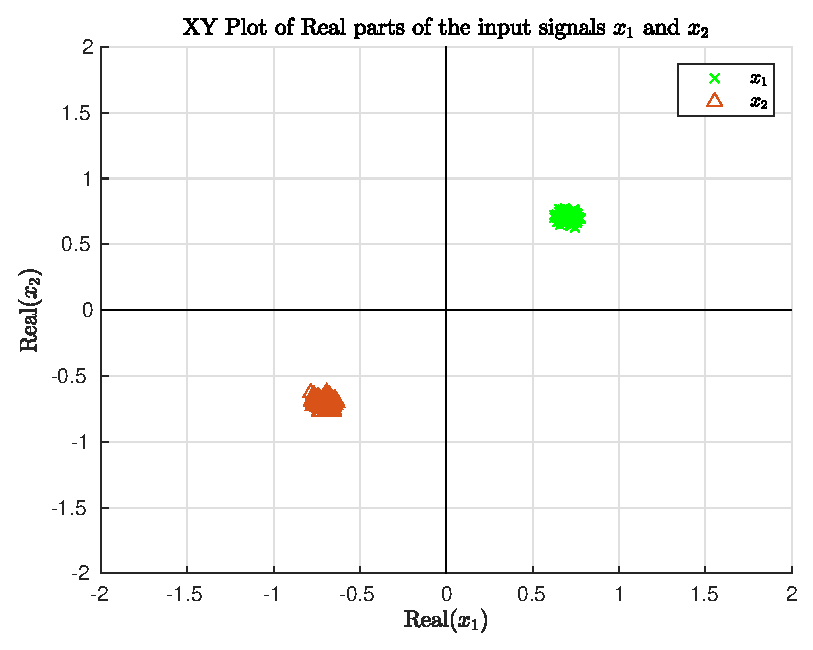
\includegraphics[width=\linewidth]{images/INNxn.eps}
    \caption{XY plot of the real parts of the input signals $x_1$ and $x_2$ with noise}
    \label{fig:INNxn}
\end{figure}

The Figure \ref{fig:INNyn} shows the received channel estimates $y_1 = h_{11}$ and $y_2 = h_{22}$. As power of this signal is highly attenuated as the air interface leads to a lot of losses. The phase shift in the various samples, represents the channel distortion effects.

\begin{figure}[H]
    \centering
    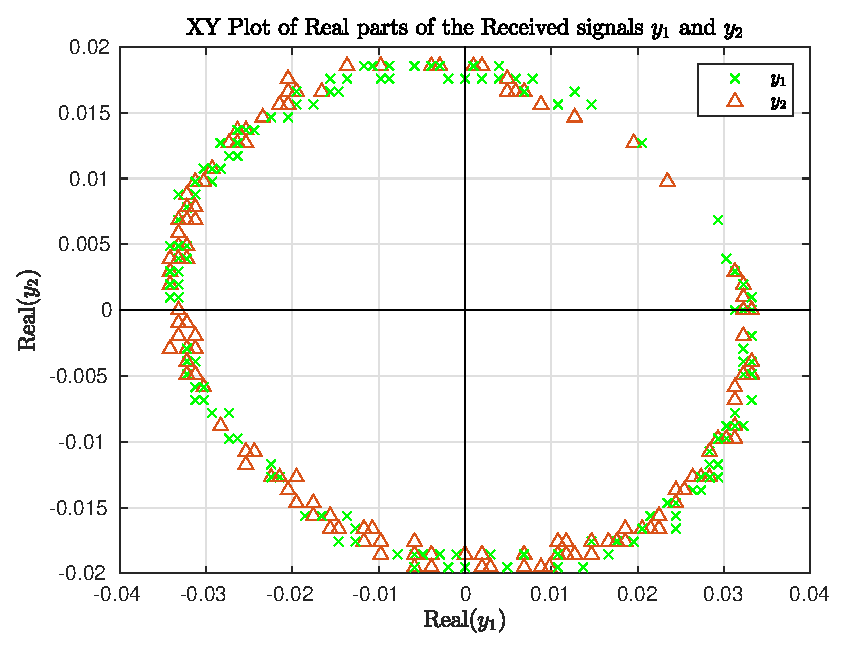
\includegraphics[width=\linewidth]{images/INNyn.eps}
    \caption{XY plot of the real parts of the received signals $y_1$ and $y_2$}
    \label{fig:INNyn}
\end{figure}

The Figure \ref{fig:INNyResult} is the output of the INN which estimates the signals $y$ based on the training data the neural network was fed with. On clustering the input and the estimated data in each of the 4 quarters of the XY plot, it was found that the detection accuracy was close to $\textbf{22}\%$.

It is to be noted that only one pair of input data namely +$\frac{1}{\sqrt{2}}$,-$\frac{1}{\sqrt{2}}$ was available instead of all 4 possibilities namely $\pm \frac{1}{\sqrt{2}}$,$\pm \frac{1}{\sqrt{2}}$. This was due to the fact that the CRS symbols chosen as the $(x,y)$ transmit and receive pair (as mentioned earlier) are in fact a predefined sequence as per the LTE standard.

One particular reason for the low detection rate could potentially be because of the complexity of the channel on the one hand and the complexity of the neural network on the otherhand. It is possible to achieve better results with some fine tuning of the neural network.

\begin{figure}[H]
    \centering
    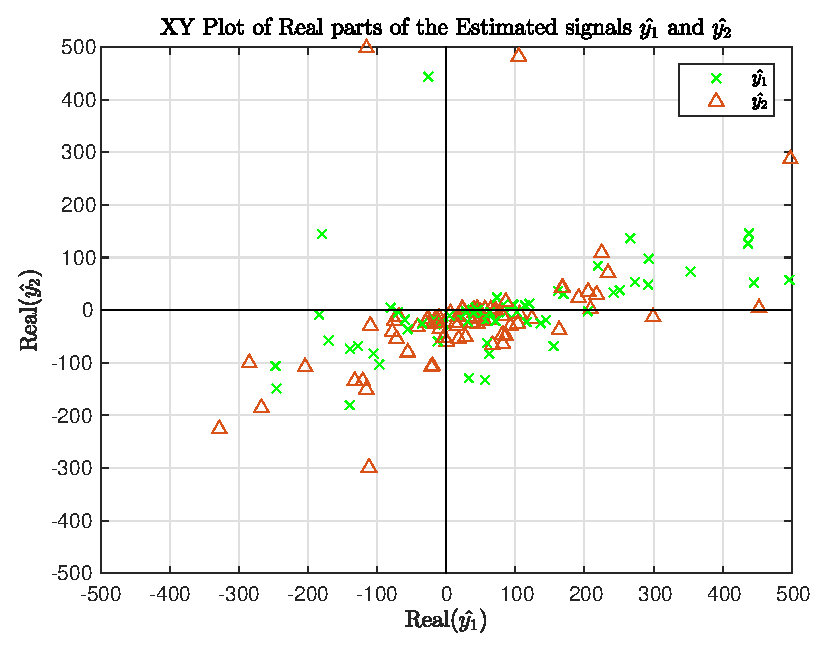
\includegraphics[width=\linewidth]{images/INNResult.eps}
    \caption{XY plot of the real parts of the INN Estimated signals $\hat{y_1}$ and $\hat{y_2}$ }
    \label{fig:INNyResult}
\end{figure}
